\documentclass[conference]{IEEEtran}
\IEEEoverridecommandlockouts
% ---- packages -------------------------------------------------------------
\usepackage[T1]{fontenc}
\usepackage{cite}
\usepackage{amsmath,amssymb,amsfonts}
\usepackage{graphicx}
\usepackage{textcomp}
\usepackage{xcolor}
\usepackage{booktabs}
\usepackage{array}
\usepackage{url}
\usepackage{tikz}
\usetikzlibrary{arrows.meta,positioning}
\usepackage{pgfplots}
\pgfplotsset{compat=1.16}
\def\BibTeX{{\rm B\kern-.05em{\sc i\kern-.025em b}\kern-.08em T\kern-.1667em\lower.7ex\hbox{E}\kern-.125emX}}
% Placeholder box for screenshots that are not supplied (keeps the project compilable without image files).
\newcommand{\figplaceholder}[3]{\fbox{\parbox[c][#1][c]{#2}{\centering\footnotesize #3}}}

\begin{document}

\title{VisionRL: Camera-Based Visual Navigation Using Deep Reinforcement Learning in Unity}

\author{\IEEEauthorblockN{[Student Name 1]}
\IEEEauthorblockA{Department of [Department]\\
[Institution]\\
[City, Country]\\
[email1@example.edu]}
\and
\IEEEauthorblockN{[Student Name 2]}
\IEEEauthorblockA{Department of [Department]\\
[Institution]\\
[City, Country]\\
[email2@example.edu]}
\and
\IEEEauthorblockN{[Student Name 3]}
\IEEEauthorblockA{Department of [Department]\\
[Institution]\\
[City, Country]\\
[email3@example.edu]}
% Add or delete \and blocks to match the number of authors.
}

\maketitle

\begin{abstract}
Reinforcement-learning agents that act directly on camera images are attractive because they need no hand-crafted state features, yet it is easy to build a benchmark in which an agent appears to use vision while actually exploiting a regularity of the task. This paper presents VisionRL, a controlled Unity environment and training pipeline for camera-based navigation with proximal policy optimization (PPO) and the Unity ML-Agents toolkit. A blue robot must reach a green exit in an 8 $\times$ 8 grid room containing twelve static obstacles. The policy receives only one 84 $\times$ 84 RGB top-down camera frame, with no vector observations and no ray sensors, and chooses one of four discrete moves. A preliminary fixed-exit version proved solvable by a policy that ignores the image, so the exit is randomized among 27 border cells, six of which are held out of training. We also describe a rendering fault, caused by Unity's GPU Resident Drawer, that left camera frames stale, and the fidelity test that exposed it and verified its fix (100\% agreement over 6,000 transitions). After 200,000 PPO steps the final policy reached the exit in 98.0\% of 200 episodes (95\% CI 95.0--99.2\%), compared with 16.5\% for the best image-blind baseline and 11.0\% when the camera was blanked. Executed by Unity's own inference engine, it succeeded in 98.0\% of 200 episodes and in 88.0\% of 100 episodes on held-out exits. Limitations include a single training seed, a single room layout and one difficult held-out exit.
\end{abstract}

\begin{IEEEkeywords}
deep reinforcement learning, proximal policy optimization, visual navigation, Unity ML-Agents, camera-blanking ablation, ONNX
\end{IEEEkeywords}


\section{Introduction}
Reinforcement learning (RL) studies how an agent can learn to act by trial and error so as to maximize cumulative reward \cite{sutton2018}. Combining RL with deep neural networks allowed agents to learn control policies directly from raw pixels, first on Atari games \cite{mnih2013atari,mnih2015dqn} and later in three-dimensional navigation tasks in which an agent must find a goal from images \cite{zhu2017target,mirowski2017navigate}. Game engines have become a practical way to build such tasks cheaply and safely: the Unity ML-Agents toolkit exposes a Unity scene as a learning environment that can be trained with a Python library \cite{juliani2018unity,mlagents_repo}.

Reporting that an agent ``learned from vision'' requires more than a high success rate. Deep RL results are sensitive to implementation details and evaluation practice \cite{henderson2018matters,engstrom2020implementation}, and agents can overfit to a fixed level or exploit a regularity that has nothing to do with the intended skill \cite{cobbe2019quantifying}. A navigation task in which the goal never moves can, for example, be solved by a policy that ignores its camera and simply drifts toward the goal's fixed location. This risk materialized in the present project: in an early fixed-exit version of the room, a policy trained with PPO reached the exit in all 200 test episodes, but so did a policy that ignored the image and sampled actions from a fixed probability vector (Section~\ref{sec:fixed}).

This paper presents VisionRL, a small but carefully validated environment and pipeline for camera-based navigation in Unity. A robot in an 8 $\times$ 8 room must reach a green exit while avoiding twelve obstacles. The only observation is one 84 $\times$ 84 RGB image from a fixed top-down camera; the positions of the robot and of the exit are never given to the policy as numbers. The exit is placed at a different border cell in every episode, so success requires locating it in the image.

\textbf{Problem statement.} Given only an 84 $\times$ 84 RGB frame at each step, learn a policy over four discrete grid moves that takes a robot from a random start cell to a randomly placed exit within 48 actions, and demonstrate, with controlled baselines, that its success depends on the camera input.

The objectives of the project were to:

\begin{enumerate}
\item build a Unity room environment with visual-only observations, explicit configurable rewards and verified episode logic;
\item randomize the exit so that image-blind policies are defeated, and quantify this with baselines;
\item train a PPO policy with Unity ML-Agents and export it in the ONNX format;
\item evaluate it with confidence intervals, a camera-blanking ablation and held-out exit positions; and
\item validate inference inside Unity and verify that the camera frames faithfully represent the simulation state.
\end{enumerate}

The main contributions are:

\begin{itemize}
\item a visual-only navigation environment with randomized and held-out exits, and a reward function audited exhaustively for exploitable positive loops;
\item baseline-driven evidence that the final policy depends on the camera: 98.0\% success with the camera, 11.0\% with the camera blanked, and 16.5\% for the best image-blind baseline;
\item documentation of a rendering fault (stale camera frames) caused by the GPU Resident Drawer, together with a reusable fidelity test that measures agreement between frames and simulation state; and
\item a reproducible train--export--infer pipeline validated with Unity's own inference engine.
\end{itemize}

The remainder of the paper reviews related work (Section~\ref{sec:lit}), describes the system and methodology (Section~\ref{sec:method}), the experimental design (Section~\ref{sec:design}), the rendering fault (Section~\ref{sec:fault}), the results (Section~\ref{sec:results}), reproducibility (Section~\ref{sec:repro}) and conclusions (Section~\ref{sec:concl}).


\section{Literature Review}\label{sec:lit}

\subsection{Reinforcement Learning and Policy-Gradient Methods}
In the standard formulation an agent interacts with a Markov decision process and seeks a policy that maximizes the expected discounted return \cite{sutton2018}. Policy-gradient methods optimize the policy directly. Trust Region Policy Optimization (TRPO) constrains each update to a region in which a surrogate objective is a reliable approximation \cite{schulman2015trpo}, and Generalized Advantage Estimation (GAE) reduces the variance of advantage estimates through a parameter $\lambda$ that trades bias for variance \cite{schulman2016gae}. Asynchronous advantage actor--critic (A3C) showed that actor--critic methods can be trained stably with parallel workers \cite{mnih2016a3c}. Proximal Policy Optimization (PPO) replaces the trust-region constraint with a clipped surrogate objective, which permits several epochs of minibatch updates on each batch of experience while keeping the new policy close to the old one \cite{schulman2017ppo}. Its simplicity and robustness made it a default choice in many toolkits, although later studies showed that code-level details strongly influence its behavior \cite{engstrom2020implementation,andrychowicz2021what}.


\subsection{Deep Reinforcement Learning from Pixels}
Deep Q-networks learned to play Atari games from raw frames using convolutional networks \cite{mnih2013atari,mnih2015dqn}. Learning from images is sample-inefficient because the network must discover useful visual features from a sparse reward signal. Later work addresses this with augmentation of the observed frames \cite{kostrikov2021drq} or with auxiliary contrastive objectives \cite{laskin2020curl}. VisionRL does not use such additions. It studies how far a standard PPO agent with a small convolutional encoder can go when the observation is small (84 $\times$ 84) and the task is simple but deliberately constructed so that the image is necessary.


\subsection{Visual Navigation and Embodied-AI Simulators}
Target-driven visual navigation trains an agent to reach a goal specified by an image in indoor scenes \cite{zhu2017target}. Auxiliary depth-prediction and loop-closure tasks help agents navigate complex mazes from pixels \cite{mirowski2017navigate}, while cognitive mapping and planning builds an explicit spatial memory from egocentric views \cite{gupta2017cmp}. Simulators such as Habitat \cite{savva2019habitat} and AI2-THOR \cite{kolve2017ai2thor}, and game-based platforms such as DeepMind Lab \cite{beattie2016dmlab} and ViZDoom \cite{kempka2016vizdoom}, provide the environments for this research. Distributed PPO has been shown to learn near-perfect point-goal navigation in photorealistic scenes given very large amounts of experience \cite{wijmans2020ddppo}, and the consistent evaluation of embodied agents is itself a topic of study \cite{anderson2018evaluation}. These systems are far richer than the room studied here. VisionRL is intentionally a small, fully inspectable setting in which every claim about visual dependence can be tested against exact ground truth.


\subsection{Simulation Platforms and Unity ML-Agents}
OpenAI Gym standardized the interface between RL algorithms and environments \cite{brockman2016gym}. The Unity platform for intelligent agents \cite{juliani2018unity} and its open-source ML-Agents toolkit \cite{mlagents_repo} let developers define an agent, its sensors and its actions in a Unity scene and train it with a Python trainer built on PyTorch \cite{paszke2019pytorch}. A trained policy can be exported in the ONNX format \cite{onnx} and executed inside Unity by a neural-network inference engine, which removes the need for Python at run time. The exported file can also be run outside Unity with ONNX Runtime \cite{onnxruntime}, which this work uses for scripted evaluation.


\subsection{Reward Shaping, Generalization and Evaluation Practice}
Sparse rewards make exploration hard. Potential-based shaping adds a term of the form $\gamma\Phi(s') - \Phi(s)$ to the reward and provably leaves the set of optimal policies unchanged \cite{ng1999shaping}. VisionRL uses this form with the shortest-path distance to the exit as the potential. Generalization in RL is commonly measured by training on one set of levels and testing on another \cite{cobbe2019quantifying,cobbe2020procgen}, and randomization of the environment is a widely used way to avoid overfitting to one configuration \cite{tobin2017domain}. We follow this idea by randomizing the exit and withholding some exit positions. Because RL results can vary strongly between seeds \cite{henderson2018matters}, statistical reporting matters, and recent work recommends interval estimates over point estimates \cite{agarwal2021precipice}. We report Wilson score intervals for success proportions \cite{wilson1927,brown2001}, which behave well for small samples and for proportions close to 0 or 1.


\subsection{Positioning of This Work}
Existing work concentrates on large, realistic or procedurally generated worlds. The contribution here is complementary: a compact environment with exhaustive ground truth, baselines designed to refute the claim that the agent uses vision, and an explicit check that the camera frames delivered to the policy are faithful to the simulation state, a failure mode that is easy to overlook.


\section{System Design and Methodology}\label{sec:method}

\subsection{Overview and Architecture}
Fig.~\ref{fig:arch} shows the system. A Unity scene contains the room, the robot and a fixed top-down camera. At every decision step the ML-Agents camera sensor renders the camera view to an 84 $\times$ 84 RGB image and passes it to the policy. The policy returns one of four discrete actions, which the environment logic converts into a one-cell move. The environment then returns a reward and a termination flag. During training these are consumed by the PPO trainer, a Python process that communicates with the Unity player through the ML-Agents interface and updates the network. When training ends, the trainer exports the network as an ONNX file, which Unity can run directly through its inference engine with no trainer attached. The game logic (positions, collisions, rewards and termination) is implemented as plain C\# classes separated from the Unity scene, so that it can be tested exhaustively without rendering. The policy never receives these quantities.

\begin{figure*}[!t]
\centering
\resizebox{0.97\textwidth}{!}{%
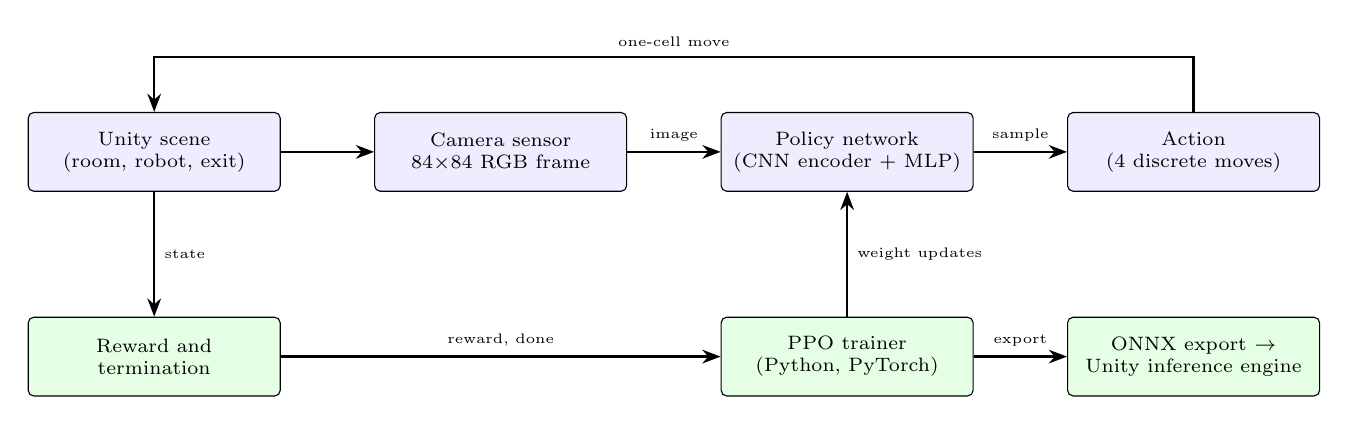
\begin{tikzpicture}[
  box/.style={draw, rounded corners=2pt, align=center, font=\scriptsize, minimum height=1.0cm, minimum width=3.2cm, fill=blue!7},
  gbox/.style={box, fill=green!10},
  arr/.style={->, >=Stealth, thick},
  lab/.style={font=\tiny, align=center}]
\node[box] (env) at (0,0) {Unity scene\\(room, robot, exit)};
\node[box] (cam) at (4.4,0) {Camera sensor\\84$\times$84 RGB frame};
\node[box] (pol) at (8.8,0) {Policy network\\(CNN encoder + MLP)};
\node[box] (act) at (13.2,0) {Action\\(4 discrete moves)};
\draw[arr] (env) -- (cam);
\draw[arr] (cam) -- node[above,lab]{image} (pol);
\draw[arr] (pol) -- node[above,lab]{sample} (act);
\draw[arr] (act.north) -- ++(0,0.7) -| node[pos=0.25,above,lab]{one-cell move} (env.north);
\node[gbox] (rew) at (0,-2.6) {Reward and\\termination};
\node[gbox] (trn) at (8.8,-2.6) {PPO trainer\\(Python, PyTorch)};
\node[gbox] (onx) at (13.2,-2.6) {ONNX export $\rightarrow$\\Unity inference engine};
\draw[arr] (env) -- node[right,lab]{state} (rew);
\draw[arr] (rew) -- node[above,lab]{reward, done} (trn);
\draw[arr] (trn) -- node[right,lab]{weight updates} (pol);
\draw[arr] (trn) -- node[above,lab]{export} (onx);
\end{tikzpicture}}
\caption{System architecture of VisionRL. Top row: the closed perception--action loop between the Unity scene, the camera sensor, the policy network and the grid move. Bottom row: reward and termination feed the PPO trainer, which updates the policy and finally exports it as an ONNX file for Unity's inference engine.}
\label{fig:arch}
\end{figure*}


\subsection{Environment}
The room is a grid of 8 $\times$ 8 cells, each one world unit wide, enclosed by four solid walls and containing twelve static obstacles (Fig.~\ref{fig:room}). The agent is a low-poly blue-and-white robot modelled from Unity primitives, with cyan sensor details and a clear front direction (Fig.~\ref{fig:robot}). Its visual model is a child object, so the appearance can be changed without touching the learning code. The exit is shown as a bright green floor marker on a border cell together with a green door slab in the adjacent wall. The floor is a graphite checkerboard with subtle grid lines, lit by one shadow-casting directional light so that walls and obstacles are readable. The robot and the exit use flat unlit materials so that their colors stay constant. Obstacle tops are deliberately much lighter than the floor so that they remain distinguishable at 84 $\times$ 84 pixels.

Movement is grid-aligned: each action moves the robot exactly one cell. A move into a wall or an obstacle leaves the robot in place and still counts as a step. The agent root object carries all ML-Agents components and the only collider; the robot model has no colliders, so it cannot interfere with the logic.

The camera is fixed, orthographic and looks straight down, so the whole room, the walls and the exit are visible in every frame. At 84 $\times$ 84 pixels one cell is about nine pixels wide. In the frames we measured, the robot's blue parts cover roughly 13 to 28 pixels and the exit marker more than 100 green pixels (Fig.~\ref{fig:obs}). This is a global, allocentric view, not a first-person view.

\begin{figure}[!t]
\centering
%% To use the real image, upload it to a figures/ folder and replace the next line with:
% \includegraphics[width=0.92\columnwidth]{figures/stage4-room-overview.png}
\figplaceholder{3.0cm}{0.92\columnwidth}{\textbf{PLACEHOLDER} -- insert: \texttt{stage4-room-overview.png}}
\caption{The randomized-exit EscapeRoom scene: graphite floor with grid lines, four walls, twelve obstacles, the blue robot and the green exit marker. (Replace with an oblique Scene-view screenshot.)}
\label{fig:room}
\end{figure}

\begin{figure}[!t]
\centering
%% To use the real image, upload it to a figures/ folder and replace the next line with:
% \includegraphics[width=0.92\columnwidth]{figures/stage3-robot-front.png}
\figplaceholder{3.0cm}{0.92\columnwidth}{\textbf{PLACEHOLDER} -- insert: \texttt{stage3-robot-front.png}}
\caption{The low-poly robot built from Unity primitives: blue and white body, upper sensor head with a cyan lens on the forward (+Z) side, and four wheels.}
\label{fig:robot}
\end{figure}

\begin{figure*}[!t]
\centering
%% To use the real image, upload it to a figures/ folder and replace the next line with:
% \includegraphics[width=0.95\textwidth]{figures/stage8-camera-exits-montage.png}
\figplaceholder{3.4cm}{0.95\textwidth}{\textbf{PLACEHOLDER} -- insert: \texttt{stage8-camera-exits-montage.png}}
\caption{Actual 84 $\times$ 84 RGB observations (enlarged with nearest-neighbour scaling) for exits on the north, north-east, west and south sides. The policy sees only such images.}
\label{fig:obs}
\end{figure*}


\subsection{Observation and Action Spaces}
The policy receives exactly one observation: the 84 $\times$ 84 RGB image from the ML-Agents camera sensor (single frame, no stacking, no grayscale conversion). The vector-observation size is zero, and no ray-perception or grid sensor is attached. The robot and exit coordinates never enter the policy. Coordinates are used only inside the environment for movement, resets and reward computation.

The action space is one discrete branch with four actions: forward (+Z), backward ($-$Z), left ($-$X) and right (+X). One decision is requested at every simulation step.


\subsection{Reward and Termination}
Rewards are configurable fields of the environment (Table~\ref{tab:reward}). An episode ends successfully when the robot enters the exit cell and ends unsuccessfully after 48 actions. In addition to these terms we use potential-based shaping \cite{ng1999shaping} with the shortest-path length $d(s)$ to the exit (found by breadth-first search) as the potential, so that the reward at step $t$ is given by Eq. (\ref{eq:reward}):

\begin{equation}
\label{eq:reward}
\begin{split}
r_t &= r_{\text{step}} + b_t\, r_{\text{block}} + \mathbb{1}[\text{exit}]\, r_{\text{exit}} + \mathbb{1}[\text{timeout}]\, r_{\text{timeout}} \\
&\quad + \gamma\,\Phi(s_{t+1}) - \Phi(s_t), \qquad \Phi(s) = -0.05\, d(s)
\end{split}
\end{equation}

where $b_t$ is one if the move was blocked and zero otherwise, and $\Phi$ is zero in terminal states. The discount $\gamma = 0.99$ equals the PPO discount.

\begin{table}[!t]
\caption{Reward components of the randomized-exit task.}
\label{tab:reward}
\centering\footnotesize\renewcommand{\arraystretch}{1.12}
\begin{tabular}{@{}>{\raggedright\arraybackslash}p{3.5cm}>{\raggedright\arraybackslash}p{3.7cm}@{}}
\toprule
Component & Value \\ \midrule
Every action ($r_{\text{step}}$) & $-$0.01 \\
Blocked move, extra ($r_{\text{block}}$) & $-$0.02 \\
Entering the exit ($r_{\text{exit}}$) & +1.0 \\
Timeout after 48 actions ($r_{\text{timeout}}$) & $-$1.0 \\
Shaping potential & $\Phi(s) = -0.05\,d(s)$, $\gamma = 0.99$ \\
Resulting step reward, moving closer & +0.0405 to +0.0465 \\
Resulting step reward, blocked & $-$0.0290 to $-$0.0230 \\
Resulting step reward, moving away & $-$0.0590 to $-$0.0530 \\
\bottomrule
\end{tabular}
\end{table}

Because shaping with $\gamma < 1$ is not exactly neutral when returns are summed without discounting, we audited the reward exhaustively (Table~\ref{tab:audit}). In all 5,508 combinations of exit, start cell and action, every step that does not bring the robot closer to the exit is negative. Only a step that reduces the path distance is positive, and a two-step back-and-forth loop never pays. The shaping scale 0.05 was chosen so that the per-step leak, $(1-\gamma)\cdot 0.05 \cdot d_{\max} \approx 0.007$ for $d_{\max} = 14$, stays below the 0.01 step penalty. In the fixed-exit prototype, an earlier scale of 0.1 allowed a small positive net reward (+0.06 over 40 steps) for oscillating far from the exit, which is why it was reduced.

\begin{table}[!t]
\caption{Reward and task-design audit (exhaustive checks and Monte-Carlo estimates, 48-action limit).}
\label{tab:audit}
\centering\footnotesize\renewcommand{\arraystretch}{1.12}
\begin{tabular}{@{}>{\raggedright\arraybackslash}p{4.6cm}>{\raggedright\arraybackslash}p{2.6cm}@{}}
\toprule
Check & Result \\ \midrule
Largest reward of a non-progress step & $-$0.0230 \\
Smallest reward of a progress step & +0.0405 \\
Best return of a two-step back-and-forth loop & $-$0.0065 \\
Always-forward/back/left/right policies: valid pairs solved & 22 of 3,440 (0.6\%) \\
Uniform random policy, success (4,000 episodes) & 7.5\% \\
Fixed-probability blind policy, success (4,000 episodes) & 15.1\% \\
Forward/right 50/50 policy, success (4,000 episodes) & 10.9\% \\
\bottomrule
\end{tabular}
\end{table}


\subsection{Exit Randomization and Held-Out Split}\label{sec:exit}
At each reset the environment first chooses an exit uniformly from the eligible set and then a start cell uniformly from the free cells that are not the exit and whose shortest-path distance to the exit is at least six steps. The eligible exits are the 27 non-obstacle cells on the border of the room, and a breadth-first search verifies that every free cell can reach each of them. The start-distance rule removes trivial episodes: the optimal route then has 6 to 14 steps and averages about 8.5 over all valid exit--start pairs. The candidates are sorted by coordinates and every fourth one (index 3 modulo 4) is withheld from training. This gives 21 training exits and six held-out exits at (0,3), (1,0), (3,0), (5,0), (7,0) and (7,4), where coordinates are (column, row) counted from the south-west corner. The exit marker and the door slab are moved together with the logical exit at every reset. Automated tests verified that the logical and visual states agree over 400 consecutive resets, and that exits occur on all four sides of the room. All random choices come from a seeded generator controlled by a reset-seed parameter, so a given seed reproduces the same sequence of (exit, start) pairs.


\subsection{Policy Network and PPO Training}
We use the PPO trainer of the ML-Agents Python package with its default small convolutional visual encoder, followed by two fully connected layers of 128 units, a four-way softmax policy output and a separate value estimate. Table~\ref{tab:hyper} lists the hyperparameters, which are taken from the project's configuration file. They are the values already used in the project's earlier experiments and were not tuned for this task. Training used the environment parameter that restricts exits to the 21 training exits, so the six held-out exits never appeared during training. The final run used seed 42 and 200,000 steps, and the trainer reported 1,658.6 s of elapsed time (about 27.6 minutes) on the CPU. The Unity player ran headless in batch mode with a 256 $\times$ 256 window and a time scale of 20.

\begin{table}[!t]
\caption{PPO training configuration (ML-Agents).}
\label{tab:hyper}
\centering\footnotesize\renewcommand{\arraystretch}{1.12}
\begin{tabular}{@{}>{\raggedright\arraybackslash}p{3.5cm}>{\raggedright\arraybackslash}p{3.7cm}@{}}
\toprule
Parameter & Value \\ \midrule
Algorithm & PPO, extrinsic reward only \\
Learning rate & $3\times 10^{-4}$, linear decay \\
Batch size / buffer size & 128 / 2,048 \\
Epochs per update & 3 \\
Clipping $\epsilon$ & 0.2 (linear decay) \\
GAE $\lambda$ & 0.95 \\
Entropy coefficient $\beta$ & 0.005 (linear decay) \\
Discount $\gamma$ & 0.99 \\
Time horizon & 64 \\
Visual encoder & default small CNN \\
Hidden units $\times$ layers & 128 $\times$ 2 \\
Input normalization & off \\
Training steps & 200,000 \\
Seed / device & 42 / CPU \\
\bottomrule
\end{tabular}
\end{table}


\subsection{Export and Unity Inference}
At the end of training the trainer writes the policy as an ONNX file of about 1.5 MB. The graph takes the image tensor (batch $\times$ 3 $\times$ 84 $\times$ 84) and an action-mask tensor and returns two action outputs: a sampled action, produced inside the graph by drawing from the softmax probabilities, and a deterministic action equal to the arg-max. Unity's inference engine runs this graph on the CPU through the Burst backend. By default Unity uses the sampled output, which matches the policy used in training. The final policy is nearly deterministic in practice, with a mean maximum action probability of 0.973 on 300 real frames. In the earlier fixed-exit model the deterministic output always returned ``forward'', because its probability distribution did not depend on the image; this was an early symptom of the image blindness discussed in Section~\ref{sec:fixed}. The Unity scene assigns the model to the agent with behavior type Default: when a Python trainer is attached the agent trains, otherwise it runs the assigned model, so the same scene serves for training and for inference.


\subsection{Implementation Environment}
Table~\ref{tab:specs} lists the software and hardware used. The ML-Agents Unity package 4.0.0 needed a one-line compatibility change to compile under Unity 6.6 (a helper for a different environment type that this project does not use), and the original file was backed up.

\begin{table}[!t]
\caption{System specifications.}
\label{tab:specs}
\centering\footnotesize\renewcommand{\arraystretch}{1.12}
\begin{tabular}{@{}>{\raggedright\arraybackslash}p{3.0cm}>{\raggedright\arraybackslash}p{4.2cm}@{}}
\toprule
Item & Specification \\ \midrule
Computer & MacBook Air, Apple M3 (ARM64), macOS \\
Game engine & Unity 6.6 (6000.6.5f1), Universal Render Pipeline 17.6.0 \\
Unity ML-Agents package & 4.0.0 (embedded, with the compatibility change above) \\
Inference in Unity & Unity Inference Engine package 2.6.1 (ML-Agents requires at least 2.2.1), Burst CPU backend \\
Python trainer & Python 3.10.12; mlagents and mlagents\_envs 1.2.0.dev0 (built from the ML-Agents release\_23 sources) \\
Deep-learning library & PyTorch 2.2.2 (CPU) \\
Evaluation tools & ONNX Runtime 1.19.2; NumPy 1.23.5; gRPC 1.51.1 \\
Camera sensor & 84 $\times$ 84 RGB, one frame, PNG-compressed transport \\
\bottomrule
\end{tabular}
\end{table}


\section{Experimental Design}\label{sec:design}
The experiments follow the workflow in Fig.~\ref{fig:workflow}. The environment tests and the observation-fidelity gate come first, training starts only after both have passed, and the exported model is evaluated in Python and then inside Unity.

\begin{figure}[!t]
\centering
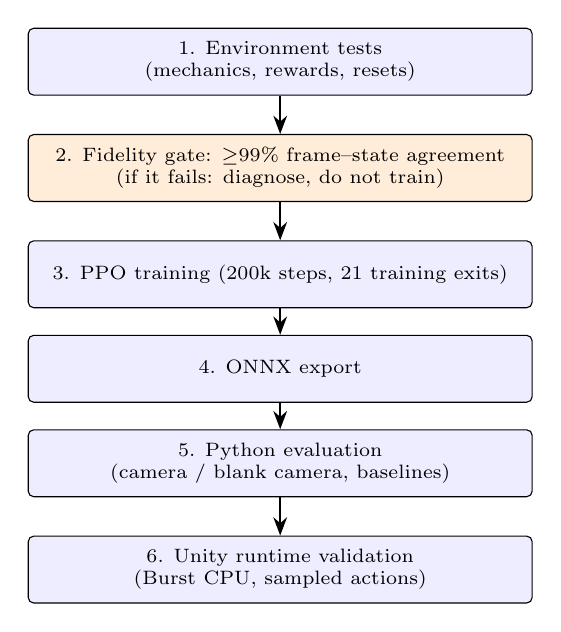
\begin{tikzpicture}[
  box/.style={draw, rounded corners=2pt, align=center, font=\scriptsize, minimum height=0.85cm, minimum width=6.4cm, fill=blue!7},
  gate/.style={box, fill=orange!15},
  arr/.style={->, >=Stealth, thick}]
\node[box]  (a) at (0,0)    {1. Environment tests\\(mechanics, rewards, resets)};
\node[gate] (b) at (0,-1.35) {2. Fidelity gate: $\geq$99\% frame--state agreement\\(if it fails: diagnose, do not train)};
\node[box]  (c) at (0,-2.7) {3. PPO training (200k steps, 21 training exits)};
\node[box]  (d) at (0,-3.9) {4. ONNX export};
\node[box]  (e) at (0,-5.1) {5. Python evaluation\\(camera / blank camera, baselines)};
\node[box]  (f) at (0,-6.45) {6. Unity runtime validation\\(Burst CPU, sampled actions)};
\foreach \p/\q in {a/b,b/c,c/d,d/e,e/f} \draw[arr] (\p) -- (\q);
\end{tikzpicture}
\caption{Workflow of the project. Training starts only after the environment tests and the observation-fidelity gate have passed; the exported model is evaluated first in Python and then inside Unity.}
\label{fig:workflow}
\end{figure}


\subsection{Baseline Policies}
Two baselines ignore the image: (i) a uniform random policy and (ii) a fixed-probability policy that samples every action from a constant distribution (forward 0.4838, backward 0.0195, left 0.1214, right 0.3753), which is the distribution learned by the earlier fixed-exit model. The second is the strongest image-blind baseline among those we measured. Policies that always choose one fixed direction succeed in only 22 of 3,440 valid exit--start pairs (0.6\%).


\subsection{Camera-Blanking Ablation}
To test whether the policy uses the image, the camera input is replaced by an image that contains no room. In the Python evaluation a constant background-colored frame is fed to the network; in Unity the camera's culling mask is set to nothing, so the sensor renders only the background color. The game itself continues unchanged. If the policy relies on the camera, its success should fall to the level of the image-blind baselines.


\subsection{Evaluation Protocol}
All policies are evaluated on the same sequence of (exit, start) pairs, produced by reset seed 9001, with exits drawn from all 27 eligible cells and sampled actions for the learned policies. The final model was evaluated for 200 episodes with the camera and for 200 episodes with the camera blanked. The baselines and the 50,000-step checkpoint come from earlier 500-episode runs with the same seed; their first 200 episodes are the same (exit, start) pairs as in the new runs, so they are reused without re-running. Success proportions are reported with 95\% Wilson score intervals \cite{wilson1927,brown2001}. A paired comparison counts the episodes won by one policy and lost by the other. An episode is a success only if the robot enters the exit before the 48-action limit; otherwise it is a timeout.


\subsection{Held-Out Exit Testing}
Held-out exits are selected with the environment parameter that restricts exits to the six withheld cells. The 50,000-step checkpoint was evaluated on 300 such episodes in Python, together with the two baselines. The final model was tested on 100 held-out episodes in Unity.


\subsection{Unity Runtime Evaluation}
The final model was also run through Unity's own inference engine in batch Play Mode on a copy of the project, with no Python trainer attached, reproducing the same episode sequence (reset seed 9001). The test first verifies that the active policy is the inference-engine policy, that the assigned model is the final ONNX file, that sampled inference is on, and that the agent has a single 84 $\times$ 84 RGB camera sensor with vector-observation size zero and no ray sensors. The agent then acts without any keyboard input. Three conditions were run: all exits with the camera (200 episodes), held-out exits only (100 episodes) and all exits with the camera blanked (200 episodes). This was not a live Editor window or a rebuilt standalone player.


\subsection{Observation-Fidelity Validation}
A data-collection script drives the player with a uniform random policy through the ML-Agents Python interface and stores every frame, action and reward. The robot and exit cells are recovered from the pixels (blue and green regions). Ground truth is obtained by replaying the executed actions through the game rules from the first frame of each episode; in the corrected player this replay reproduces the logged rewards exactly, which validates it. Four checks follow: (a) the frame shows the true robot cell; (b) the replayed reward equals the real reward; (c) the frame changes when the robot truly moves; and (d) the robot's position in the frame stays unchanged when a move is blocked. A player is accepted only if each of these is at least 99\%.


\section{The Rendering Fault and Observation Fidelity}\label{sec:fault}
A first training run on the randomized-exit task (run 01) did not learn. For 109,445 steps its mean episode reward stayed between about $-$0.7 and $-$1.0, and its 50,000-step checkpoint succeeded in 68 of 500 episodes (13.6\%, 95\% CI 10.9--16.9\%), which is indistinguishable from the 14.8\% (74 of 500) of the fixed-probability blind policy. Instead of simply training for longer, we inspected the data the policy actually received. Frames were pixel-identical for long stretches although the logged rewards showed that the robot kept moving. The robot's cell in the frame changed only 46 times in 9,000 frames, and the frame showed the true robot cell in 100\% of first steps but in only 19.5\% of steps 2--10 and 5.7\% of steps 11--48 (Table~\ref{tab:fidelity} and Fig.~\ref{fig:stale}). The exit marker, which changes only at a reset, was updated correctly. The agent therefore could not learn where it was from the image.

\begin{figure*}[!t]
\centering
%% To use the real image, upload it to a figures/ folder and replace the next line with:
% \includegraphics[width=0.95\textwidth]{figures/stage8-diag-frames-19-26.png}
\figplaceholder{3.4cm}{0.95\textwidth}{\textbf{PLACEHOLDER} -- insert: \texttt{stage8-diag-frames-19-26.png}}
\caption{Evidence of stale frames in the faulty player: consecutive observations 19--26 of one episode. After step 21 the images are identical although the robot kept moving (as shown by the logged rewards).}
\label{fig:stale}
\end{figure*}

\textbf{Diagnosis and fix.} The player rendered through the Universal Render Pipeline with the GPU Resident Drawer enabled (the setting \texttt{m\_GPUResidentDrawerMode} was 1 in the render-pipeline asset). A player built with the setting disabled produced faithful frames, whereas the otherwise identical player with it enabled did not. We did not isolate the exact mechanism inside Unity. A plausible explanation is that the drawer refreshes the transforms of moving renderers only at frame boundaries, whereas the trainer advances the simulation many times per rendered frame. The fix was a one-line change from 1 to 0 in the PC pipeline asset, applied after backing up the original (the mobile asset already had the drawer disabled), and a new player was built. Because this is a project-wide setting, the regression checks of all scenes were re-run and passed: 33 of 33 play-mode checks and 1,596 mechanics assertions for the original grid scene, 31 edit-mode and 26 play-mode checks for the fixed-exit room, and 34 edit-mode and 12 play-mode checks for the randomized-exit room.

\begin{table}[!t]
\caption{Observation fidelity of the player before and after the fix.}
\label{tab:fidelity}
\centering\footnotesize\renewcommand{\arraystretch}{1.12}
\begin{tabular}{@{}>{\raggedright\arraybackslash}p{2.6cm}>{\raggedright\arraybackslash}p{2.0cm}>{\raggedright\arraybackslash}p{2.0cm}@{}}
\toprule
Measure & Drawer on (faulty) & Drawer off (fixed) \\ \midrule
Transitions / episodes & 9,000 / 194 & 6,000 / 129 \\
Frame shows true robot cell & 10.4\% & 100\% \\
Reward replay agreement & 32.4\% & 100\% \\
Frame changes on true moves & 0.6\% & 100\% \\
Unchanged on blocked moves & 99.7\% (trivial) & 100\% \\
Exit stable within episode & 99.7\% & 100\% \\
Robot-cell changes seen & 46 & 4,163 \\
\bottomrule
\end{tabular}
\end{table}

The 99.7\% in the faulty player for blocked moves is trivial, because the frames almost never changed at all. The check was repeated on fresh data (3,000 transitions, 63 episodes; all measures 100\%) immediately before the final training run.

\textbf{Lesson.} Unit tests of the environment logic and checks that the robot is visible in the frame both passed while the observation was wrong. Only a test that compares the frame with the true state at every step exposed the fault. For camera-based RL we therefore recommend an automated fidelity test as an acceptance gate before any training.


\section{Results and Discussion}\label{sec:results}

\subsection{Training Behavior}
Fig.~\ref{fig:curve} shows the mean episode reward reported by the trainer. In the corrected player (run 02) the reward started near $-$0.94, crossed zero at about 30,000 steps, reached 1.17 at 70,000 steps and then stayed at about 1.35 (1.346 to 1.360 between 110,000 and 200,000 steps). A plateau near 1.35 is consistent with near-optimal play: from the reward formula, the return of an optimal episode is about 1.25 for a six-step route and 1.5 for a twelve-step route. In the faulty player (run 01) the reward stayed between $-$0.7 and $-$1.0 until the run was stopped. A training curve is a statistic of the stochastic policy on training exits, so it is not by itself evidence of visual navigation; the evaluations below are.

\begin{figure}[!t]
\centering
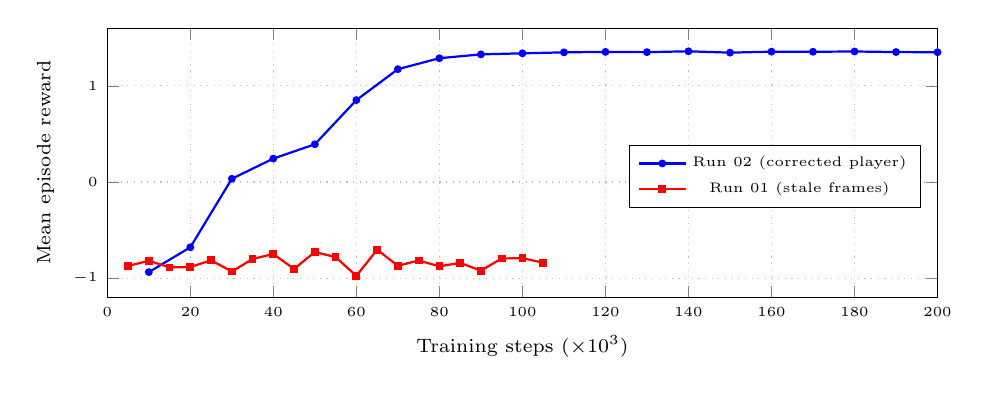
\begin{tikzpicture}
\begin{axis}[width=\columnwidth, height=5.0cm, xlabel={Training steps ($\times 10^{3}$)}, ylabel={Mean episode reward},
  xmin=0, xmax=200, ymin=-1.2, ymax=1.6, grid=both, grid style={dotted}, tick label style={font=\tiny}, label style={font=\scriptsize},
  legend style={font=\tiny, at={(0.98,0.45)}, anchor=east}]
\addplot[blue, thick, mark=*, mark size=1pt] coordinates {(10,-0.937) (20,-0.679) (30,0.034) (40,0.244) (50,0.393) (60,0.852) (70,1.174) (80,1.288) (90,1.328) (100,1.339) (110,1.349) (120,1.354) (130,1.351) (140,1.360) (150,1.346) (160,1.356) (170,1.355) (180,1.358) (190,1.352) (200,1.350)};
\addlegendentry{Run 02 (corrected player)}
\addplot[red, thick, mark=square*, mark size=1pt] coordinates {(5,-0.873) (10,-0.819) (15,-0.888) (20,-0.884) (25,-0.814) (30,-0.931) (35,-0.800) (40,-0.749) (45,-0.904) (50,-0.728) (55,-0.781) (60,-0.976) (65,-0.704) (70,-0.871) (75,-0.816) (80,-0.877) (85,-0.841) (90,-0.922) (95,-0.795) (100,-0.792) (105,-0.839)};
\addlegendentry{Run 01 (stale frames)}
\end{axis}
\end{tikzpicture}
\caption{Mean episode reward during training. Run 02 (corrected player) learns; run 01 (stale camera frames) stays near the level of random behavior. Run 01 was stopped at about 105,000 steps.}
\label{fig:curve}
\end{figure}


\subsection{Python Evaluation}
Table~\ref{tab:python} and Fig.~\ref{fig:bars} compare all policies on the same 200 episodes. The final model reached the exit in 196 of 200 episodes (98.0\%, 95\% CI 95.0--99.2\%), with a mean episode length of 9.6 steps and a mean of 8.8 steps on successful episodes, close to the estimated optimal average of about 8.5 steps. The best image-blind baseline reached 16.5\% (12.0--22.3\%) and the uniform random policy 5.5\% (3.1--9.6\%); the intervals of the final model and of the baselines do not overlap. In a paired comparison on the identical episodes, the final model succeeded in 163 episodes that the blind policy lost, and the blind policy never succeeded where the final model failed.

\begin{table*}[!t]
\caption{Python evaluation (reset seed 9001, all 27 exits, same 200 episodes for every row, sampled actions). Intervals are 95\% Wilson score intervals.}
\label{tab:python}
\centering\footnotesize\renewcommand{\arraystretch}{1.12}
\begin{tabular}{@{}lrrrr@{}}
\toprule
Policy & Success & 95\% CI & Timeouts & Mean length \\ \midrule
Uniform random & 11/200 (5.5\%) & 3.1--9.6\% & 94.5\% & 47.1 \\
Best blind policy & 33/200 (16.5\%) & 12.0--22.3\% & 83.5\% & 43.7 \\
50k checkpoint, camera & 145/200 (72.5\%) & 65.9--78.2\% & 27.5\% & 30.5 \\
50k checkpoint, blank camera & 15/200 (7.5\%) & 4.6--12.0\% & 92.5\% & 47.2 \\
\textbf{Final model, camera} & \textbf{196/200 (98.0\%)} & \textbf{95.0--99.2\%} & \textbf{2.0\%} & \textbf{9.6} \\
Final model, blank camera & 22/200 (11.0\%) & 7.4--16.1\% & 89.0\% & 46.7 \\
\bottomrule
\end{tabular}
\end{table*}

\begin{figure}[!t]
\centering
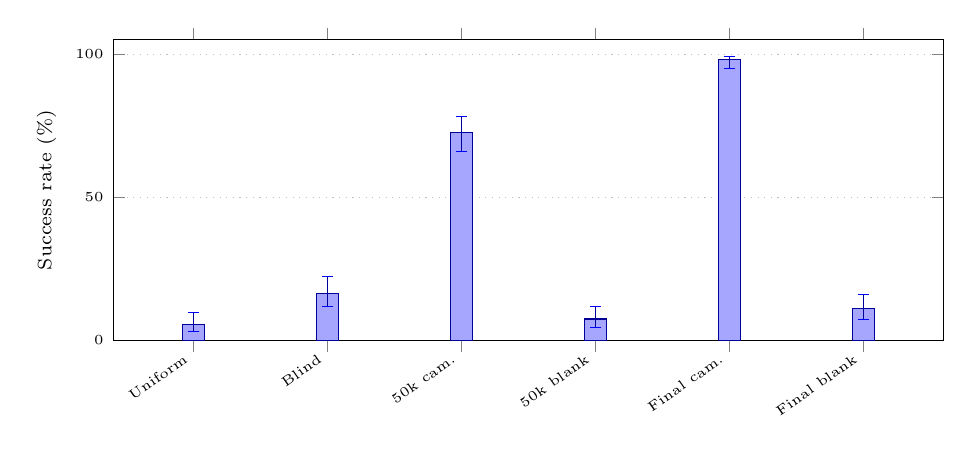
\begin{tikzpicture}
\begin{axis}[ybar, width=\columnwidth, height=5.4cm, bar width=8pt, ymin=0, ymax=105, ylabel={Success rate (\%)},
  symbolic x coords={Uniform,Blind,C50k,B50k,Fcam,Fblank}, xtick=data,
  xticklabels={Uniform,Blind,50k cam.,50k blank,Final cam.,Final blank},
  xticklabel style={rotate=35, anchor=east, font=\tiny}, yticklabel style={font=\tiny}, ylabel style={font=\scriptsize},
  enlarge x limits=0.12, ymajorgrids, grid style={dotted}]
\addplot+[fill=blue!35, draw=blue!60!black, error bars/.cd, y dir=both, y explicit] coordinates {(Uniform,5.5) += (0,4.1) -= (0,2.4) (Blind,16.5) += (0,5.8) -= (0,4.5) (C50k,72.5) += (0,5.7) -= (0,6.6) (B50k,7.5) += (0,4.5) -= (0,2.9) (Fcam,98.0) += (0,1.2) -= (0,3.0) (Fblank,11.0) += (0,5.1) -= (0,3.6)};
\end{axis}
\end{tikzpicture}
\caption{Success rate (Python evaluation, 200 episodes) with 95\% Wilson intervals. Blanking the camera reduces the final model to the level of the image-blind baselines.}
\label{fig:bars}
\end{figure}


\subsection{Camera Dependence}
Blanking the camera reduces the final model from 98.0\% to 11.0\% (intervals 95.0--99.2\% and 7.4--16.1\%), a level comparable to the best blind baseline (12.0--22.3\%). The 50,000-step checkpoint behaves the same way (72.5\% with the camera and 7.5\% without). This strongly supports the conclusion that the policy relies on the image to find the exit. Because the frame contains the robot, the obstacles and the exit, the ablation does not separate which visual cues are used; it shows that the information needed for navigation is carried by the image and not by a position-independent action preference. The action statistics support this reading. In Unity, the final policy's action mix over all-exit episodes was 27\% forward, 29\% backward, 20\% left and 24\% right, depending on the situation, whereas the fixed-exit model, which ignored the image, used a constant mix of 49\%, 2\%, 12\% and 38\%.


\subsection{Unity Runtime Results}
Table~\ref{tab:unity} reports the test with Unity's inference engine. These are Unity results and are distinct from the Python results above. In the verification step the active policy was the inference-engine policy, the assigned model was the final ONNX file, sampled inference was on, and the agent had a single 84 $\times$ 84 RGB camera sensor, vector-observation size zero and no ray sensors. No Unity errors or exceptions were logged. With the camera, the success on all exits (196 of 200) equals the Python result on the same episode sequence. Blanking the camera gave 12.0\% in Unity and 11.0\% in Python; the two use different blanking methods, and the difference is within sampling error.

\begin{table*}[!t]
\caption{Unity runtime evaluation of the final model (Unity inference engine, Burst CPU, sampled actions, batch Play Mode, reset seed 9001).}
\label{tab:unity}
\centering\footnotesize\renewcommand{\arraystretch}{1.12}
\begin{tabular}{@{}lrrrrr@{}}
\toprule
Condition & Episodes & Success & 95\% CI & Timeouts & Mean length \\ \midrule
All exits, camera & 200 & 196 (98.0\%) & 95.0--99.2\% & 2.0\% & 9.5 \\
Held-out exits, camera & 100 & 88 (88.0\%) & 80.2--93.0\% & 12.0\% & 14.2 \\
All exits, camera blanked & 200 & 24 (12.0\%) & 8.2--17.2\% & 88.0\% & 46.3 \\
\bottomrule
\end{tabular}
\end{table*}


\subsection{Generalization to Held-Out Exits}
On the six exits never seen in training, the final model succeeded in 88 of 100 Unity episodes (Table~\ref{tab:heldout}). Five of the six exits were solved in all 85 attempts combined, whereas the exit at (0,3), on the west wall next to an obstacle, was solved in only 3 of 15 attempts. The only four failures in the 200 all-exit Unity episodes were also at this exit. We did not investigate the cause; one untested hypothesis is that the approach to this exit is constrained by the neighboring obstacle and resembles no training situation. The earlier 50,000-step checkpoint scored 75.0\% (225 of 300; 95\% CI 69.8--79.6\%) on held-out exits in Python, against 5.7\% (17 of 300; 3.6--8.9\%) for the uniform random policy and 0.7\% (2 of 300; 0.2--2.4\%) for the fixed-probability blind policy.

\begin{table}[!t]
\caption{Final model, Unity, held-out exits only (100 episodes). Coordinates are (column, row).}
\label{tab:heldout}
\centering\footnotesize\renewcommand{\arraystretch}{1.12}
\begin{tabular}{@{}lrr@{}}
\toprule
Held-out exit & Wall & Successes \\ \midrule
(0,3) & west & 3 / 15 \\
(1,0) & south & 16 / 16 \\
(3,0) & south & 15 / 15 \\
(5,0) & south & 19 / 19 \\
(7,0) & south-east corner & 17 / 17 \\
(7,4) & east & 18 / 18 \\
\bottomrule
\end{tabular}
\end{table}


\subsection{Preliminary Fixed-Exit Experiment}\label{sec:fixed}
In the earlier fixed-exit room (exit in the north-east corner, 128-action limit, 30,000 training steps), the trained policy reached the exit in 200 of 200 Unity episodes and in 200 of 200 Python episodes on each of two seeds. A fixed-probability policy that never looked at the image also achieved 200 of 200 on both seeds, with mean lengths of 17.2 and 16.7 steps against 16.8 and 16.2 for the model, and with the camera blanked the model still succeeded in 194 of 200 episodes (97.0\%). Across 34 distinct real frames its action probabilities changed by at most 0.0005. Success rate alone therefore could not show vision in that task, which is the reason for randomizing the exit. These early runs used a player built before the rendering fix; the blind-policy result does not depend on the frames.


\subsection{Limitations}
The following limitations should be kept in mind.

\begin{itemize}
\item Only one training seed (42) was run, so seed-to-seed variability is unknown.
\item There is one fixed room layout with twelve obstacles; only the exit and start positions are randomized.
\item The camera is a fixed top-down view of a small 8 $\times$ 8 grid with discrete one-cell moves, which is far from first-person navigation or real robotics. The work does not address object detection, semantic segmentation or navigation in real environments.
\item One held-out exit, (0,3), was not solved reliably (3 of 15).
\item The Unity validation ran in batch Play Mode on a project copy. It was not a live Editor window, and the previously built standalone players predate the final model assignment and were not re-validated with it.
\item Sampled-action evaluation is not bit-reproducible, because the sampling inside the ONNX graph is unseeded; the (exit, start) sequence is reproducible.
\item The 50,000-step and baseline rows reuse the first 200 episodes of longer runs, and the Python blank-camera control approximates the blanked Unity camera with a constant frame.
\item The exact internal cause of the rendering fault was not isolated; only its effect and its remedy were verified.
\end{itemize}


\section{Reproducibility and Deployment}\label{sec:repro}
The environment logic and the agent are implemented in two C\# classes (\texttt{RoomWorld} and \texttt{RoomAgent}), and the scene is generated by an Editor script, so the room can be recreated from source. The final model is \url{results/visionrl-random-exit-02/VisionRL/VisionRL-200008.onnx} (1,515,126 bytes). It is byte-identical to the checkpoint \url{VisionRL-199996.onnx} exported a moment earlier and to the \url{VisionRL.onnx} copy in the run directory. The training and evaluation commands were:

{\footnotesize
\begin{verbatim}
mlagents-learn Training/ppo-random-exit.yaml
  --env Builds/EscapeRoomRandomExit-fixed.app
  --run-id visionrl-random-exit-02 --seed 42
  --env-args -batchmode -screen-fullscreen 0
  -screen-width 256 -screen-height 256

python Training/evaluate.py --env <player>
  --model <model.onnx> --actions sampled
  --exit-set 0 --episodes 200 --seed 9001
\end{verbatim}}

The training configuration differs from the project's original configuration file only in the number of steps (200,000 instead of 300,000) and in the parameter that restricts exits to the training set; the original file, the earlier scenes and all earlier results were preserved. The fidelity scripts and the evaluation reports are stored with the project.

For deployment, the final ONNX file is assigned to the agent in the randomized-exit scene with behavior type Default, the Burst CPU inference device and sampled inference. Opening the scene and pressing Play makes the robot navigate to the exit without keyboard input; the decision period of the agent can be raised to slow it down for viewing. Standalone players built before this assignment were not re-validated with the final model. The project source and reports are available at [repository URL to be added by the authors].


\section{Conclusion and Future Work}\label{sec:concl}
VisionRL shows, in a controlled Unity environment, that a PPO agent can learn to navigate from a single 84 $\times$ 84 RGB camera frame to a randomly placed exit. The final policy reached the exit in 98.0\% of 200 episodes (95\% CI 95.0--99.2\%), against 16.5\% for the best image-blind baseline, and in 98.0\% of 200 episodes when run by Unity's own inference engine. With the camera blanked its success fell to 11.0\% in Python and 12.0\% in Unity, and it also solved 88\% of 100 Unity episodes on exits never seen in training. Together, these results support vision-dependent reinforcement learning in this environment. The study also shows the value of validating observation fidelity: a rendering fault that left the camera frames stale made training impossible, and only a test that compares frames with the true simulation state revealed it.

The conclusions are limited to one training seed, one room layout, a fixed overhead camera and one held-out exit that was not solved reliably. Future work includes (i) repeating training with several seeds and reporting aggregate statistics \cite{agarwal2021precipice}; (ii) randomizing the obstacle layout in addition to the exit \cite{cobbe2020procgen}; (iii) adding image augmentation \cite{kostrikov2021drq} or contrastive representation learning \cite{laskin2020curl}; (iv) moving to an egocentric camera with frame stacking and richer scenes; (v) analyzing the failures at the held-out exit and identifying which visual cues the policy uses; (vi) re-validating a rebuilt standalone player with the final model; and (vii) studying transfer beyond simulation, where domain randomization may help \cite{tobin2017domain}.


\section*{Acknowledgment}
The authors thank [supervisor name and institution] for guidance and facilities. [Edit or remove as appropriate.]


% Bibliography embedded so that this file compiles on its own (no references.bib needed).
\begin{thebibliography}{34}
\bibitem{sutton2018}
R. S. Sutton and A. G. Barto, \textit{Reinforcement Learning: An Introduction}, 2nd ed. Cambridge, MA, USA: MIT Press, 2018.
\bibitem{mnih2013atari}
V. Mnih, K. Kavukcuoglu, D. Silver, A. Graves, I. Antonoglou, D. Wierstra, and M. Riedmiller, ``Playing Atari with Deep Reinforcement Learning,'' arXiv:1312.5602, 2013.
\bibitem{mnih2015dqn}
V. Mnih, K. Kavukcuoglu, D. Silver, et al., ``Human-level control through deep reinforcement learning,'' \textit{Nature}, vol. 518, no. 7540, pp. 529--533, 2015, doi: 10.1038/nature14236.
\bibitem{zhu2017target}
Y. Zhu, R. Mottaghi, E. Kolve, et al., ``Target-driven Visual Navigation in Indoor Scenes using Deep Reinforcement Learning,'' in \textit{Proc. IEEE Int. Conf. Robotics and Automation (ICRA)}, 2017, arXiv:1609.05143.
\bibitem{mirowski2017navigate}
P. Mirowski, R. Pascanu, F. Viola, et al., ``Learning to Navigate in Complex Environments,'' in \textit{Proc. Int. Conf. Learning Representations (ICLR)}, 2017, arXiv:1611.03673.
\bibitem{juliani2018unity}
A. Juliani, V. P. Berges, E. Teng, et al., ``Unity: A General Platform for Intelligent Agents,'' arXiv:1809.02627, 2018.
\bibitem{mlagents_repo}
Unity Technologies, ``Unity {ML-Agents} Toolkit.'' GitHub repository. [Online]. Available: \url{https://github.com/Unity-Technologies/ml-agents}
\bibitem{henderson2018matters}
P. Henderson, R. Islam, P. Bachman, J. Pineau, D. Precup, and D. Meger, ``Deep Reinforcement Learning That Matters,'' in \textit{Proc. AAAI Conf. Artificial Intelligence}, 2018, arXiv:1709.06560.
\bibitem{engstrom2020implementation}
L. Engstrom, A. Ilyas, S. Santurkar, et al., ``Implementation Matters in Deep Policy Gradients: A Case Study on {PPO} and {TRPO},'' in \textit{Proc. Int. Conf. Learning Representations (ICLR)}, 2020, arXiv:2005.12729.
\bibitem{cobbe2019quantifying}
K. Cobbe, O. Klimov, C. Hesse, T. Kim, and J. Schulman, ``Quantifying Generalization in Reinforcement Learning,'' in \textit{Proc. 36th Int. Conf. Machine Learning (ICML)}, 2019, arXiv:1812.02341.
\bibitem{schulman2015trpo}
J. Schulman, S. Levine, P. Moritz, M. Jordan, and P. Abbeel, ``Trust Region Policy Optimization,'' in \textit{Proc. 32nd Int. Conf. Machine Learning (ICML)}, 2015, arXiv:1502.05477.
\bibitem{schulman2016gae}
J. Schulman, P. Moritz, S. Levine, M. Jordan, and P. Abbeel, ``High-Dimensional Continuous Control Using Generalized Advantage Estimation,'' in \textit{Proc. Int. Conf. Learning Representations (ICLR)}, 2016, arXiv:1506.02438.
\bibitem{mnih2016a3c}
V. Mnih, A. P. Badia, M. Mirza, et al., ``Asynchronous Methods for Deep Reinforcement Learning,'' in \textit{Proc. 33rd Int. Conf. Machine Learning (ICML)}, 2016, arXiv:1602.01783.
\bibitem{schulman2017ppo}
J. Schulman, F. Wolski, P. Dhariwal, A. Radford, and O. Klimov, ``Proximal Policy Optimization Algorithms,'' arXiv:1707.06347, 2017.
\bibitem{andrychowicz2021what}
M. Andrychowicz, A. Raichuk, et al., ``What Matters for On-Policy Deep Actor-Critic Methods? A Large-Scale Study,'' in \textit{Proc. Int. Conf. Learning Representations (ICLR)}, 2021, arXiv:2006.05990.
\bibitem{kostrikov2021drq}
I. Kostrikov, D. Yarats, and R. Fergus, ``Image Augmentation Is All You Need: Regularizing Deep Reinforcement Learning from Pixels,'' in \textit{Proc. Int. Conf. Learning Representations (ICLR)}, 2021, arXiv:2004.13649.
\bibitem{laskin2020curl}
M. Laskin, A. Srinivas, and P. Abbeel, ``{CURL}: Contrastive Unsupervised Representations for Reinforcement Learning,'' in \textit{Proc. 37th Int. Conf. Machine Learning (ICML)}, 2020, arXiv:2004.04136.
\bibitem{gupta2017cmp}
S. Gupta, J. Davidson, S. Levine, R. Sukthankar, and J. Malik, ``Cognitive Mapping and Planning for Visual Navigation,'' in \textit{Proc. IEEE Conf. Computer Vision and Pattern Recognition (CVPR)}, 2017, arXiv:1702.03920.
\bibitem{savva2019habitat}
M. Savva, A. Kadian, O. Maksymets, et al., ``Habitat: A Platform for Embodied {AI} Research,'' in \textit{Proc. IEEE/CVF Int. Conf. Computer Vision (ICCV)}, 2019, arXiv:1904.01201.
\bibitem{kolve2017ai2thor}
E. Kolve, R. Mottaghi, W. Han, et al., ``{AI2-THOR}: An Interactive {3D} Environment for Visual {AI},'' arXiv:1712.05474, 2017.
\bibitem{beattie2016dmlab}
C. Beattie, J. Z. Leibo, D. Teplyashin, et al., ``{DeepMind Lab},'' arXiv:1612.03801, 2016.
\bibitem{kempka2016vizdoom}
M. Kempka, M. Wydmuch, G. Runc, J. Toczek, and W. Jaskowski, ``{ViZDoom}: A {Doom}-based {AI} Research Platform for Visual Reinforcement Learning,'' in \textit{Proc. IEEE Conf. Computational Intelligence and Games (CIG)}, 2016, arXiv:1605.02097.
\bibitem{wijmans2020ddppo}
E. Wijmans, A. Kadian, A. Morcos, et al., ``{DD-PPO}: Learning Near-Perfect {PointGoal} Navigators from 2.5 Billion Frames,'' in \textit{Proc. Int. Conf. Learning Representations (ICLR)}, 2020, arXiv:1911.00357.
\bibitem{anderson2018evaluation}
P. Anderson, A. Chang, D. S. Chaplot, et al., ``On Evaluation of Embodied Navigation Agents,'' arXiv:1807.06757, 2018.
\bibitem{brockman2016gym}
G. Brockman, V. Cheung, L. Pettersson, J. Schneider, J. Schulman, J. Tang, and W. Zaremba, ``{OpenAI Gym},'' arXiv:1606.01540, 2016.
\bibitem{paszke2019pytorch}
A. Paszke, S. Gross, F. Massa, et al., ``{PyTorch}: An Imperative Style, High-Performance Deep Learning Library,'' in \textit{Advances in Neural Information Processing Systems (NeurIPS)}, 2019, arXiv:1912.01703.
\bibitem{onnx}
ONNX Project Contributors, ``{ONNX}: Open Neural Network Exchange.'' [Online]. Available: \url{https://onnx.ai}
\bibitem{onnxruntime}
ONNX Runtime Developers, ``{ONNX Runtime}.'' GitHub repository. [Online]. Available: \url{https://github.com/microsoft/onnxruntime}
\bibitem{ng1999shaping}
A. Y. Ng, D. Harada, and S. Russell, ``Policy Invariance Under Reward Transformations: Theory and Application to Reward Shaping,'' in \textit{Proc. 16th Int. Conf. Machine Learning (ICML)}, 1999, pp. 278--287.
\bibitem{cobbe2020procgen}
K. Cobbe, C. Hesse, J. Hilton, and J. Schulman, ``Leveraging Procedural Generation to Benchmark Reinforcement Learning,'' in \textit{Proc. 37th Int. Conf. Machine Learning (ICML)}, 2020, arXiv:1912.01588.
\bibitem{tobin2017domain}
J. Tobin, R. Fong, A. Ray, J. Schneider, W. Zaremba, and P. Abbeel, ``Domain Randomization for Transferring Deep Neural Networks from Simulation to the Real World,'' in \textit{Proc. IEEE/RSJ Int. Conf. Intelligent Robots and Systems (IROS)}, 2017, arXiv:1703.06907.
\bibitem{agarwal2021precipice}
R. Agarwal, M. Schwarzer, P. S. Castro, A. Courville, and M. G. Bellemare, ``Deep Reinforcement Learning at the Edge of the Statistical Precipice,'' in \textit{Advances in Neural Information Processing Systems (NeurIPS)}, 2021, arXiv:2108.13264.
\bibitem{wilson1927}
E. B. Wilson, ``Probable Inference, the Law of Succession, and Statistical Inference,'' \textit{Journal of the American Statistical Association}, vol. 22, no. 158, pp. 209--212, 1927.
\bibitem{brown2001}
L. D. Brown, T. T. Cai, and A. DasGupta, ``Interval Estimation for a Binomial Proportion,'' \textit{Statistical Science}, vol. 16, no. 2, pp. 101--133, 2001, doi: 10.1214/ss/1009213286.
\end{thebibliography}

\end{document}
